\documentclass[12pt]{article}
\usepackage[utf8]{inputenc}
\usepackage[top=0.75in, bottom=0.75in, left=0.75in, right=0.75in, headheight=15pt]{geometry}
\usepackage{amsmath, amssymb, amsthm, graphicx, hyperref, enumerate, multirow,  multicol, tikz, centernot, cancel, forest, lipsum, mathtools, bm, esvect, fancyhdr, esdiff, float, parskip, comment}

\DeclareMathSymbol{*}{\mathbin}{symbols}{"01} % change * to /cdot inside math
% \begingroup % let only this align, etc. break across pages
% \allowdisplaybreaks
% \begin{align}
%     ....
% \end{align}
% \endgroup

% \begin{figure}[H]
%     \centering
%     \includegraphics{}
%     \caption{}
%     \label{fig:}
% \end{figure}

% \texorpdfstring{$k$}{k} math inside (sub/)section label

\pagestyle{fancy}
\fancyhead[L]{Liheng Cao}
% \fancyhead[C]{center}
\fancyhead[R]{}

\title{LA HW 3} % title
\author{Liheng Cao} % name
\date{\today} % custom date else today's date

\begin{document}
\maketitle

\section{} % Q1
\begin{enumerate}[G1]
	\item \,
		\begin{enumerate}[(a)]
			\item 
				\[\mathrm{Inc} = 
					\begin{bmatrix}
						-1 & 0 & -1 & 0\\
						1 & -1 & 0 & 0\\
						0 & 1 & 1 & -1\\
						0 & 0 & 0 & 1
					\end{bmatrix}
				\]
				\[
					\Delta(G) = 
					\begin{bmatrix}
						2 & -1 & -1 & 0\\
						-1 & 2 & -1 & 0\\
						-1 & -1 & 3 & -1\\
						0 & 0 & -1 & 1
					\end{bmatrix}
				\]
				
			\item 
				\[\mathrm{Deg} = 
					\begin{bmatrix}
						2 & 0 & 0 & 0\\
						0 & 2 & 0 & 0\\
						0 & 0 & 3 & 0\\
						0 & 0 & 0 & 1
					\end{bmatrix}\]
				\[\mathrm{Adj} = 
					\begin{bmatrix}
						0 & 1 & 1 & 0\\
						1 & 0 & 1 & 0\\
						1 & 1 & 0 & 1\\
						0 & 0 & 1 & 0
					\end{bmatrix}\]
			\item The eigenvalues are the row vectors.
				\[\operatorname{eigen}(\Delta(G)) = 
					\begin{bmatrix}
						1 & 1 & -3 & 1\\
						-1 & 1 & 0 & 0\\
						-1 & -1 & 0 & 2\\
						1 & 1 & 1 & 1
					\end{bmatrix},
					[4,3,1,0]
				\]
				\[
					\operatorname{eigen}(\mathrm{Deg}) = I_4, [2,2,3,1]
				\]
				\[
					\operatorname{eigen}(\mathrm{Adj}) \approx
					\begin{bmatrix}
						1.85 & 1.85 & 2.17 & 1\\
						0.60 & 0.60 & -1.48 & 1\\
						-1 & 1 & 0 & 0\\
						-0.45 & -0.45 & 0.31 & 1
					\end{bmatrix} , 
					[-2.17, 1.48, 1, -0.311]
				\]
			
			\item Note: This question will only be answered once because it is not dependent on the graph. The Cheeger estimate tells us this. Alternatively, since the eigenvalues of a matrix are equal to that of its transpose, the eigenvalues of $ \Delta(G) $ are real and non-negative because it's the product of a matrix and it's transpose. It's like how multiplying a value by itself makes it real and non-negative.
		\end{enumerate}
	
	\item 
		\begin{enumerate}[(a)]
			\item 
				\[\mathrm{Inc} = 
					\begin{bmatrix}
						-1 &  0 &  0 &  1 & -1 &  0\\
						1  & -1 &  0 &  0 &  0 & -1\\
						0  &  1 & -1 & -1 &  0 &  0\\
						0  &  0 &  1 &  0 &  1 &  1
					\end{bmatrix}
				\]
				\[
				\Delta(G) = 
					\begin{bmatrix}
						3 & -1 & -1 & -1\\
						-1 & 3 & -1 & -1\\
						-1 & -1 & 3 & -1\\
						-1 & -1 & -1 & 3
					\end{bmatrix}
				\]
			
			\item 
				\[\mathrm{Deg}=
					\begin{bmatrix}
						3 & 0 & 0 & 0\\
						0 & 3 & 0 & 0\\
						0 & 0 & 3 & 0\\
						0 & 0 & 0 & 3
					\end{bmatrix}
				\]
				\[\mathrm{Adj}=
					\begin{bmatrix}
						0 & 1 & 1 & 1\\
						1 & 0 & 1 & 1\\
						1 & 1 & 0 & 1\\
						1 & 1 & 1 & 0
					\end{bmatrix}
				\]
				
			\item 
				\[\operatorname{eigen}(G) = 
					\begin{bmatrix}
						-1 & 0 & 0 & 1\\
						-1 & 0 & 1 & 0\\
						-1 & 1 & 0 & 0\\
						1 & 1 & 1 & 1
					\end{bmatrix}, [4,4,4,0]
				\]
				\[\operatorname{eigen}(Deg) = [1,1,1,1], [3]\]
				\[\operatorname{eigen}(Adj) = 
					\begin{bmatrix}
						1 & 1 & 1 & 1\\
						-1 & 0 & 0 & 1\\
						-1 & 0 & 1 & 0\\
						-1 & 1 & 0 & 0
					\end{bmatrix}, [3,1,1,1]
				\]
		\end{enumerate}
	
	\item 
		\begin{enumerate}[(a)]
			\item 
				\[\mathrm{Inc} = 
					\begin{bmatrix}
						-1 & 0 & 0 & 1 & -1\\
						1 & -1 & 0 & 0 & 0\\
						0 & 1 & -1 & 0 & 1\\
						0 & 0 & 1 & -1 & 0
					\end{bmatrix}
				\]
				\[\Delta(G) = 
					\begin{bmatrix}
						3 & -1 & -1 & -1\\
						-1 & 2 & -1 & 0\\
						-1 & -1 & 3 & -1\\
						-1 & 0 & -1 & 2
					\end{bmatrix}
				\]
				
			\item 
				\[\mathrm{Deg} = 
					\begin{bmatrix}
						3 & 0 & 0 & 0\\
						0 & 2 & 0 & 0\\
						0 & 0 & 3 & 0\\
						0 & 0 & 0 & 2
					\end{bmatrix}
				\]
				
				\[\mathrm{Adj} = 
					\begin{bmatrix}
						0 & 1 & 1 & 1\\
						1 & 0 & 1 & 0\\
						1 & 1 & 0 & 1\\
						1 & 0 & 1 & 0
					\end{bmatrix}
				\]
				
			\item 
				\[\operatorname{eigen}(G) = 
					\begin{bmatrix}
						-2 & 1 & 0 & 1\\
						-1 & 0 & 1 & 0\\
						0 & -1 & 0 & 1\\
						1 & 1 & 1 & 1
					\end{bmatrix}, [4,4,2,0]
				\]
				\[\operatorname{eigen}(Deg) = I_4, [3, 2 , 3, 2]
				\]
				\[
				\operatorname{eigen}(Adj) \approx
					\begin{bmatrix}
						1.28 & 1 & 1.28 & 1\\
						-0.79 & 1 & -0.78 & 1\\
						-1 & 0 & 1 & 0\\
						0 & -1 & 0 & 1
					\end{bmatrix}, [3,1,1,1]
				\]
		\end{enumerate}
\end{enumerate}
\newpage

\section{} % Q2
\begin{enumerate}[(a)]
	\item 
		\[\operatorname{eigen}(\Delta(G)) = 
		\begin{bmatrix}
			1  & 1  & -3 & 1 \\
			-1 & 1  & 0  & 0 \\
			-1 & -1 & 0  & 2 \\
			1  & 1  & 1  & 1
		\end{bmatrix},
		[4,3,1,0]
		\]
		We can see that $ 4 \geq 3 \geq 1 \ge 0 = 0 $
		
	\item 
		\begin{enumerate}[a]
			\item \[\dfrac{2 * 2}{1} = 4 > \lambda_2 = 1\]
				
			\item \[\dfrac{2 * 2}{1} = 4 > \lambda_2 = 1\]
			
			\item \[\dfrac{2*1}{1} > \lambda_2 = 1\]
		\end{enumerate}
	
	\item \[\lambda_2 \leq \dfrac{2\|\#E(V_1, V_2)\|}{\operatorname{min}\{\|V_1\|, \|V_2\|\}}\]
	
	\item The determinant of the mesh of the graph is equal to the number of spanning trees. Coefficient of T in the characteristic polynomial is equal to the number of vertices times the number of spanning trees.
\end{enumerate}

\newpage

\section{} % Q3
\begin{enumerate}[(G1)]
	\item 
		\begin{enumerate}[(a)]
			\item There are 3 trees that span the graph.
			
			\item 
				\[\Delta(G) = 
				\begin{bmatrix}
					2 & -1 & -1 & 0\\
					-1 & 2 & -1 & 0\\
					-1 & -1 & 3 & -1\\
					0 & 0 & -1 & 1
				\end{bmatrix}
				\]
				
				The characteristic polynomial is $ -12T + 19T^2 - 8T^3 + T^4 $.
				
			\item Since we only care about the zeros of this polynomial, we can multiply it by $ -1 $. So we don't need to worry about the sign. The coefficient is equal to the number of connected nodes/vertices times the number of spanning trees. $ 4 * 3 = 12 $
			
			\item The tree that omits $ e_2 $ will be used.
			
			The vector is $ [1,-1,1] $
			
			\[ \begin{bmatrix}
				3
			\end{bmatrix} \]
				
			\item The determinant is 3. They are equal.
		\end{enumerate}
	
	\item 
		\begin{enumerate}[(a)]
			\item There are 16 trees that span the graph.
			
			\item 
				\[\Delta(G) = 
				\begin{bmatrix}
					3 & -1 & -1 & -1\\
					-1 & 3 & -1 & -1\\
					-1 & -1 & 3 & -1\\
					-1 & -1 & -1 & 3
				\end{bmatrix}
				\]
			
				The characteristic polynomial is $ -64T + 48T^2 - 12T^3+T^4$.
			
			\item Since we only care about the zeros of this polynomial, we can multiply it by $ -1 $. So we don't need to worry about the sign. The coefficient is equal to the number of connected nodes/vertices times the number of spanning trees. $ 16 * 4 = 64 $
			
			\item The tree that omits the 3 sides of the triangle will be used.
			
				The vectors are $ [-1,1,-1], [-1,1,-1], [-1,1,-1] $
				\[ M = \begin{bmatrix}
					3 & -1 & -1\\
					-1 & 3 & -1\\
					-1 & -1 & 3
					\end{bmatrix} 
				\]
			
			\item The determinant is 16. They are equal.
		\end{enumerate}
	
	\item 
		\begin{enumerate}[(a)]
			\item There are 8 trees that span the graph.
			
			\item 
				\[\Delta(G) = 
					\begin{bmatrix}
						3 & -1 & -1 & -1\\
						-1 & 2 & -1 & 0\\
						-1 & -1 & 3 & -1\\
						-1 & 0 & -1 & 2
					\end{bmatrix}
				\]
				
				The characteristic polynomial is $ -21T + 32T^2 - 10T^3 + T^4$.
				
			\item Since we only care about the zeros of this polynomial, we can multiply it by $ -1 $. So we don't need to worry about the sign. The coefficient is equal to the number of connected nodes/vertices times the number of spanning trees. $ 16 * 4 = 64 $
			
			\item The tree that has the right and top edge omitted will be used. 
			
			The vectors are $ [1,1,1], [1,1,-1] $.
			\[M = \begin{bmatrix}
				3 & -1\\
				-1 & 3
			\end{bmatrix}\]
			
			\item The determinant is 8. They are equal.
		\end{enumerate}
\end{enumerate}

\newpage

\section{} % Q4
\begin{enumerate}[(a)]
	\item $ R \approx 7.66, S \approx 22.48 $. The general formulas are $ R = \dfrac{\operatorname{Sample\,Correlation}(X, Y)}{\operatorname{Sample\,Variance}(X)}, S = \bar{Y} - \bar{X}R $
	
	\item Yes. It does by definition.
	
	\item 
		\begin{figure}[H]
			\centering
			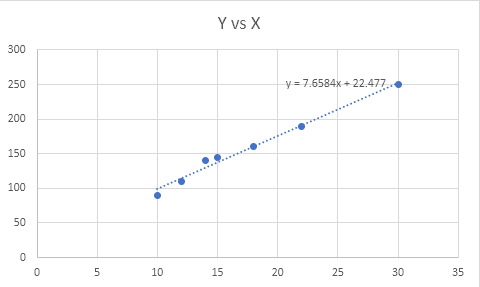
\includegraphics[width=\linewidth]{images/4c.png}
			\caption{Excel screenshot}
			\label{fig:4:c}
		\end{figure}
\end{enumerate}

\newpage

\section{} % Q5
\[A = 
\begin{bmatrix}
	10 & 12 & 14 & 15 & 18 & 22 & 30\\
	90 & 110 & 140 & 145 & 160 & 189 & 250
\end{bmatrix}
\]
Subtract $ \bar{X} $ element-wise from the first row, and subtract $ \bar{Y} $ element-wise from the second row to get $ B $.
Note: The equation had to be shrunk to fit on the page.
\begin{tiny}
	\[B =
	\begin{bmatrix}
		10 - 17.286 & 12 - 17.286 & 14 - 17.286 & 15 - 17.286 & 18 - 17.286 & 22 - 17.286 & 30 - 17.286\\
		90 - 154.857 & 110 - 154.857 & 140 - 154.857 & 145 - 154.857 & 160 - 154.857 & 189 - 154.857 & 250 - 154.857
	\end{bmatrix}
	\]
\end{tiny}

Now calculate $ BB^\intercal $
\[BB^\intercal = 
\begin{bmatrix}
	281.42 & 2155.28\\
	2155.18 & 16780.68
\end{bmatrix}
\]
This matrix's row eigenvectors are 
\[\begin{bmatrix}
	0.127 & 0.991\\
	0.991 & -0.127
\end{bmatrix}\]

Our result is $ 0.127X + 0.991Y, 0.991X 0 0.127Y $.

\newpage

\section{} % Q6
Note: the matrix $ A $ given in the hw pdf is different from the one covered in class; the difference is the value of $ A_{2,3} $. Since the matrix values covered in class results in cleaner numbers, I will be using those values.
\[A=
\begin{bmatrix}
	4 & 11 & 14\\
	8 & 7 & -2
\end{bmatrix}
\]
Decompose into the form $ U \Sigma V^\intercal $

Calculate $ A^\intercal A $
\[A^\intercal A =
\begin{bmatrix}
	80 & 100 & 40\\
	100 & 170 & 140\\
	40 & 140 & 200
\end{bmatrix}\]
Find the eigenvalues and eigenvectors. 
\[\lambda_1 = 360, \lambda_2 = 90, \lambda_3 = 0\]
\[V = 
\begin{bmatrix}
	1 & 2 & 2\\
	-2 & -1 & 2\\
	2 & -2 & 1
\end{bmatrix}\]
Find $ U $
\[ u_1 = A v_1/\sqrt{\lambda_1} = [3/\sqrt{10}, 1/\sqrt{10}]^\intercal \]
\[ u_2 = A v_2/\sqrt{\lambda_2} = [1/\sqrt{10}, -3/\sqrt{10}]^\intercal \]


\[ A = \left(\dfrac{1}{\sqrt{10}}
	\begin{bmatrix}
		3 & 1\\
		1 & -3
	\end{bmatrix}\right)
\left(\dfrac{1}{\sqrt{10}}
	\begin{bmatrix}
		6 & 0 & 0\\
		0 & 1 & 0
	\end{bmatrix}\right)
	\begin{bmatrix}
		1 & 2 & 2\\
		-2 & -1 & 2\\
		2 & -2 & 1
	\end{bmatrix}^\intercal
\]
\[= \dfrac{1}{10}
\begin{bmatrix}
	3 & 1\\
	1 & -3
\end{bmatrix}
\begin{bmatrix}
	6 & 0 & 0\\
	0 & 3 & 0
\end{bmatrix}
\begin{bmatrix}
	1 & 2 & 2\\
	-2 & -1 & 2\\
	2 & -2 & 1
\end{bmatrix}^\intercal\]


\end{document}